\documentclass[11pt]{article}
\usepackage[preprint]{acl}
\usepackage{times}
\usepackage{latexsym}
\usepackage[T1]{fontenc}
\usepackage[utf8]{inputenc}
\usepackage{microtype}
\usepackage{inconsolata}
\usepackage{graphicx}
\usepackage{booktabs}
\usepackage{amsmath}
\usepackage[capitalise,noabbrev]{cleveref}

\title{Jev versus 7B Language Models for Speech-Neuroprosthesis Rescoring:\\
A Pre-Registered Comparison in Two Participants}

\author{Gabriele Cin\`a \\ \texttt{c.gabriele.info@gmail.com}}

\begin{document}
\maketitle

\begin{abstract}
Speech neuroprostheses decode attempted speech from intracortical activity and end by rescoring
the decoder's candidate sentences with a language model of several billion parameters, the only
component that needs a GPU. A cheaper rescorer must still pick the right sentence among
near-identical candidates, and general language models asked to choose from a list in one call
answer from where a label sits rather than from the sentence. We pose rescoring as a single typed
decision served by Jev, a hosted model trained for calibrated decisions, and compare it with
OPT-6.7b and Qwen2.5-7B on identical candidate lists from two participants with amyotrophic lateral
sclerosis under two tuning protocols. On participant T15 (8.1\% first-pass word error) Jev is ahead of both 7B models
in all four comparisons and at most 0.20 points behind at the 95\% bound. A pre-registered
replication on participant T12 (19.2\% first-pass word error) meets the fixed margin in two of four
comparisons; the other two are inconclusive, with point estimates of $+0.10$ and $+0.08$ points.
Open models given the same single-call task fail because they answer from label position. Jev costs \$0.07 to
\$0.12 per thousand sentences and spends 62\,ms at the provider per call, with end-to-end latency
of 240 to 280\,ms dominated by the network.
\end{abstract}

\section{Introduction}

%TL;DR: A speech BCI ends in LLM rescoring, and that stage sets the hardware and cost.
A speech neuroprosthesis turns intracortical activity into text in three stages. A recurrent
network trained with connectionist temporal classification~\citep{graves2006ctc} emits phoneme
probabilities, a lexicon- and $n$-gram-constrained decoder turns them into a ranked list of
candidate sentences, and a language model rescores that list before the system speaks the
winner~\citep{willett2023,card2024}. This last stage is the only one that needs a
multi-billion-parameter model, so it sets the accelerator, the power budget and the cost of the
system.

%TL;DR: The stage only selects, but general LLMs fail when asked to select in one call.
The rescorer's job is selection: the answer is one of $N$ sentences already written down. One call
over the whole list is the natural form for a selector, but general language models handle it
badly: asked to choose from a list, they favour positions over
contents~\citep{tang2023psc,bito2026position}.

%TL;DR: Typed-decision models are trained for this output; none has been tested on neural decoding.
A typed-decision model is trained for exactly this output. Given a state and a question with a fixed
set of answers, it returns a probability for each answer in one pass and cannot produce anything
outside the set. Jev~\citep{typesafe2026} is such a model, served through an API. Third-party
evaluations report lower latency and cost than API-served language models on service
orchestration~\citep{li2026edge} and text annotation~\citep{ibrahim2026annotation}; none tests it on
neural decoding or against scorers on a local GPU.

%TL;DR: What we do and what we find.
We replace the rescorer of the published pipeline with Jev for two participants and compare it with
the two 7B models the stage would otherwise use, on byte-identical candidate lists. We derived the margin that
defines \emph{matches} from the first participant and fixed it, together with the full analysis, in
a public pre-registration before decoding any data from the second. \Cref{fig:forest} summarises
the outcome.

\paragraph{Contributions.}
\begin{itemize}\itemsep1pt
\item On T15, Jev is ahead of OPT-6.7b and Qwen2.5-7B in all four comparisons; on T12 the
  pre-registered test confirms two of four, and no point estimate favours a 7B model by more
  than $0.10$ points (\cref{sec:acc}).
\item Open models given the same single-call task fail on both participants: when they deviate
  from the decoder's top candidate they pick the truth 0.2--2.4\% of the time, against 15--27\% for
  Jev (\cref{sec:collapse}).
\item Jev needs no local accelerator and costs \$0.07--0.12 per thousand sentences; its latency is
  network-bound and not below a local 7B scorer (\cref{sec:cost}).
\end{itemize}
We release candidate lists, per-arm scores, latency logs, the T12 decoder code and the
pre-registration.\footnote{\url{https://github.com/gabrycina/how-much-language-model}}

\begin{figure}[t]
\centering
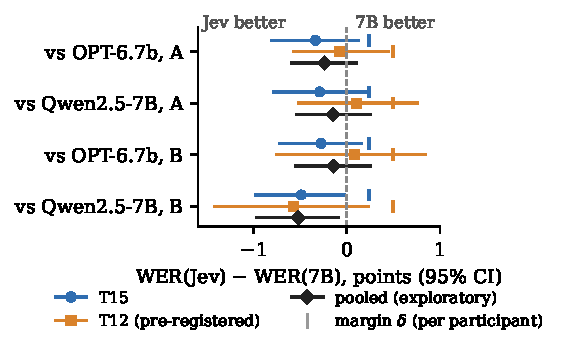
\includegraphics[width=\columnwidth]{fig_forest.pdf}
\caption{Jev minus each 7B rescorer on the test split, with paired 95\% intervals. Ticks mark each
participant's margin $\delta$. Points left of zero favour Jev.}
\label{fig:forest}
\end{figure}

\section{Related work}
\label{sec:related}

%TL;DR: BCI rescoring always uses a multi-billion-parameter model; we keep the pipeline and swap it.
\citet{willett2023} and \citet{card2024} both finish decoding with a large language model, the
latter in a system with single-digit error, as do the Brain-to-Text '24 entries~\citep{b2t24}.
Speech recognition
interpolates the first-pass score with a language model~\citep{udagawa2022} or trains the rescorer
discriminatively~\citep{xu2022rescorebert,shivakumar2023disc,yu2023lora}; discriminative training
needs more lists than a few hundred development sentences supply, so every arm here, Jev included,
runs without task-specific training.

Listwise reranking with language models suffers position bias,
which permutation self-consistency~\citep{tang2023psc} and order-invariant
architectures~\citep{bito2026invarirank} address. Self-consistency multiplies the number of calls by the
number of permutations, which removes the single-call property that motivates the typed format, so
we do not apply it; we test open models in Jev's single-call format and diagnose their failure. Prior Jev evaluations~\citep{li2026edge,ibrahim2026annotation} compare
against generation over an API; our baselines score on a local GPU, the harder comparison for
latency.

\section{Setup}
\label{sec:setup}

%TL;DR: Decoder score and combination rule.
\paragraph{Problem.} For each attempted sentence the decoder emits a list $H$ ranked by
$\ell(h) = \lambda\, a(h) + g(h)$, where $a$ is the acoustic score, $g$ the $n$-gram score and
$\lambda$ the acoustic weight. A rescorer assigns $r(h)$ to every candidate and the system speaks
\begin{equation}
  \hat h = \arg\max_{h \in H}\; (1-\alpha)\, z_H[\ell](h) + \alpha\, z_H[r](h),
\end{equation}
where $z_H$ standardises scores across the list. A \emph{per-candidate} rescorer sets $r(h)$ to the
length-normalised log-likelihood of $h$; a \emph{typed} rescorer sees the list once, with $h_i$ under
label $i$, and we set $r(h_i) = \log \max(p_i, 10^{-6})$ for its label distribution $p$.

%TL;DR: Two participants, one decoder.
\paragraph{Data and lists.} Both public datasets record a participant with amyotrophic lateral
sclerosis attempting prompted sentences. For \textbf{T15}~\citep{card2024,t15data} we use the
benchmark's validation split (1,397 sentences) and the authors' pretrained phoneme network. For
\textbf{T12}~\citep{willett2023,t12data} we use the \texttt{test} partition (877 unique sentences) and
train the public baseline network ourselves, selecting the checkpoint on held-out \texttt{train}
trials rather than on \texttt{test} as the baseline's trainer does (\cref{app:t12}). For both, the
Kaldi weighted finite-state transducer decoder~\citep{povey2011kaldi} and OpenWebText 3-gram released with the T15 benchmark
produce 100-best lists with identical options; the truth is in the list for 89\% (T15) and 71\%
(T12) of sentences. Every arm scores the same cached lists.

%TL;DR: Arms.
\paragraph{Arms.} We call each rescorer under test an \emph{arm}. OPT-6.7b~\citep{zhang2022opt} and Qwen2.5-7B~\citep{qwen2025} score every
candidate on one NVIDIA L40S. Jev (\texttt{jev-latest}, resolving to \texttt{jev-1.13.0}) receives
each list once (\cref{app:prompt}). As controls, Laya~\citep{laya2026}, an open 421M typed-decision
model, receives the identical request, and OPT-6.7b and Qwen2.5-7B receive the same task as a text
prompt, read from their next-token probability of each label.

%TL;DR: Tuning protocols and statistics.
\paragraph{Protocols and statistics.} We split each participant's sentences 30/70 into development
and test with a fixed seed (419/978 for T15, 263/614 for T12). Under protocol \textbf{A} we set
$\lambda$ to the value that minimises first-pass development error and tune $\alpha$ per arm; under
\textbf{B} we tune $\lambda$ and $\alpha$ jointly per arm. We score the test split once and report
corpus-level word error rate (WER). Arm differences are paired percentile bootstraps over test
sentences (5,000 resamples, two-sided 95\% intervals). Jev \emph{matches} a 7B model when the upper
bound on $\mathrm{WER}_{\text{Jev}} - \mathrm{WER}_{\text{7B}}$ lies below
$\delta = 0.025 \times$ the first-pass development error, which equals 0.24 points for T15 and 0.50
for T12. We chose $\delta$ after seeing T15, so T15 is exploratory; we committed the T12 analysis publicly
before decoding any T12 data (\cref{app:prereg}).

\section{Results}
\label{sec:results}


\begin{table}[t]
\centering\small
\setlength{\tabcolsep}{4pt}
\begin{tabular}{lcccc}
\toprule
& \multicolumn{2}{c}{T15 ($n$=978)} & \multicolumn{2}{c}{T12 ($n$=614)} \\
\cmidrule(lr){2-3}\cmidrule(lr){4-5}
Arm & A & B & A & B \\
\midrule
No rescoring & 8.09 & 8.09 & 19.23 & 19.23 \\
OPT-6.7b & 7.80 & 7.20$^*$ & 18.84 & 17.59$^*$ \\
Qwen2.5-7B & 7.75 & 7.42$^*$ & 18.66 & 18.24$^*$ \\
Jev & 7.46$^*$ & 6.93$^*$ & 18.76 & 17.67$^*$ \\
\bottomrule
\end{tabular}
\caption{Test word error (\%). $^*$: better than no rescoring after Holm correction over the three
arms within a protocol and participant ($p<0.05$, one-sided paired bootstrap). Full per-arm settings
in \cref{app:full}.}
\label{tab:wer}
\end{table}

\subsection{Accuracy}
\label{sec:acc}

%TL;DR: T15: Jev ahead in all four, bound 0.20.
On T15, Jev is the most accurate arm under both protocols (\cref{tab:wer}) and ahead of both 7B
models in all four comparisons, by 0.28 to 0.49 points (\cref{fig:forest}). Every interval excludes a
Jev deficit larger than 0.20 points, inside the 0.24-point margin.

%TL;DR: T12: partly confirmed; failures are width, not a deficit.
On T12, the pre-registered test confirms the margin against OPT-6.7b under protocol A (difference
$-0.08$, interval $[-0.57, +0.44]$) and against Qwen2.5-7B under protocol B ($-0.57$,
$[-1.42, +0.23]$). The other two comparisons are inconclusive: their point estimates are $+0.10$ and
$+0.08$ points, but their intervals reach $+0.75$ and $+0.84$, above the 0.50-point margin. A
plausible reading is that these failures reflect interval width on 614 noisier test sentences
rather than a deficit, since neither point estimate exceeds 0.10 points. Under
protocol B every main arm improves on no rescoring on both participants, by 0.67 to 1.64 points.

%TL;DR: Pooled and robustness.
Pooling both participants, an analysis we did not pre-register, Jev is ahead in all four comparisons
and at most 0.25 points behind at the 95\% bound. Removing test sentences whose text also occurs in
the phoneme network's training data (107 for T15, 19 for T12) leaves every point estimate at or
below $+0.03$ and widens the intervals (\cref{app:overlap}).

\subsection{The typed format needs a trained model}
\label{sec:collapse}

\begin{table}[t]
\centering\small
\setlength{\tabcolsep}{3.5pt}
\begin{tabular}{lcccccc}
\toprule
& \multicolumn{3}{c}{T15} & \multicolumn{3}{c}{T12} \\
\cmidrule(lr){2-4}\cmidrule(lr){5-7}
Typed arm & used & on A & $\neq$A & used & on A & $\neq$A \\
\midrule
Jev & 57 & 72\% & 26.6\% & 69 & 57\% & 15.1\% \\
Laya & 44 & 69\% & 2.3\% & 51 & 49\% & 2.2\% \\
Qwen2.5-7B & 31 & 28\% & 2.4\% & 25 & 4\% & 1.1\% \\
OPT-6.7b & 13 & 35\% & 0.2\% & 11 & 20\% & 0.4\% \\
\bottomrule
\end{tabular}
\caption{Typed arms before combination, all lists. \emph{used}: distinct labels chosen out of 100;
\emph{on A}: share of answers on the decoder's top candidate; $\neq$\emph{A}: how often an answer
other than A is the true sentence.}
\label{tab:collapse}
\end{table}

%TL;DR: Open models collapse; Jev's deviations carry signal on both participants.
The gain comes from the model, not from the single-call format. Given the same task, Laya and the
two 7B models in typed mode never beat no rescoring on either participant (\cref{app:full}). All four
typed arms show strong position preferences, but not for the same position. Jev and Laya place 49--72\% of
their answers on label A, the decoder's own top candidate. The open 7B models instead concentrate
on fixed positions whatever the list contains: OPT-6.7b gives 27\% of its T15 answers and 61\% of
its T12 answers to position 68, and Qwen2.5-7B gives 16\% and 26\% to position 27. What separates
the arms is what happens when they deviate from label A (\cref{tab:collapse}): Jev's other answers
are the true sentence 15--27\% of the time, the open models' 0.2--2.4\%.

\subsection{Cost and latency}
\label{sec:cost}

\begin{table}[t]
\centering\scriptsize
\setlength{\tabcolsep}{3pt}
\begin{tabular}{lcc}
\toprule
& T15 & T12 \\
\midrule
Mean candidates per list & 39 & 80 \\
Jev input tokens per list, mean & 1,631 & 2,825 \\
Jev cost per 1,000 sentences & \$0.069 & \$0.119 \\
OPT-6.7b cost per 1,000 sentences, busy L40S & \$0.029 & \$0.051 \\
GPU break-even utilisation vs.\ Jev (OPT-6.7b) & 43\% & 43\% \\
Jev median latency, scoring run (ms) & 282 & 253 \\
OPT-6.7b median latency, scoring run (ms) & 27 & 116 \\
Jev end-to-end, London client (ms) & 262 & 242 \\
Jev server time, provider proxy (ms) & 62 & 62 \\
Jev two-option request end-to-end (ms) & 253 & 221 \\
\bottomrule
\end{tabular}
\caption{Cost and latency. Token counts from the API's usage field on 140 (T15) and 60 (T12) random
test lists; GPU cost at \$1.82 per L40S-hour. Scoring-run latencies are per list from a data centre
in Finland; the London measurements pair each full request with a two-option request on the same
keep-alive connection.}
\label{tab:latency}
\end{table}

%TL;DR: Cost: cheaper per user, not per busy-GPU sentence.
Jev bills a mean 1,631 input tokens per T15 list and 2,825 per T12 list, which is \$0.069 and \$0.119
per thousand sentences. OPT-6.7b on a fully used L40S costs \$0.029 and \$0.051, so a busy GPU is
cheaper per sentence; the GPU wins only above 43\% utilisation on both participants. One user
produces a small fraction of a GPU's hourly capacity of about 36,000 to 62,000 lists: at 1,000
sentences a day Jev costs \$0.07 to \$0.12, against \$43.68 for a dedicated on-demand GPU.

%TL;DR: Latency: network-bound, not below local.
Jev answers in a median 282\,ms (T15) and 253\,ms (T12), against 27\,ms and 116\,ms for OPT-6.7b on
the local GPU. The provider's proxy reports a median 62\,ms of server time on both participants,
independent of list length, and a two-option request takes almost as long end to end as a full list
(\cref{tab:latency}). The remaining 175 to 195\,ms is transport. A co-located deployment would
approach the same order as a local 7B model, not below it; we could not test this.

\section{Conclusion}

%TL;DR: Recap and future work.
One typed decision from Jev rescores a speech neuroprosthesis's candidate list about as well as a 7B
language model that scores every candidate: ahead in all four comparisons on T15 and in the pooled
data, and within a pre-registered margin in two of four on T12, with no point estimate favouring
the 7B models by more than 0.10 points. Open models given the same task fail, so the result depends on
a model trained for the decision. The next step is an open typed-decision model of known size
trained on this task, which would let the cost and latency claims be tested on a patient's own
hardware and allow a confirmatory test with more participants.

\section*{Limitations}

%TL;DR: The limitations a reviewer should weigh.
\textbf{One closed model.} Jev's size and architecture are undisclosed, so the result shows that a
typed-decision model does this job, not why; hosted models also change over time. We release its
per-sentence label probabilities so the analysis is reproducible, though the model is not.
\textbf{Two participants, limited power.} Differences below about half a point are hard to resolve,
which is why two T12 comparisons are inconclusive. \textbf{Margin.} We derived $\delta$ from T15;
only T12 is confirmatory. \textbf{Our T12 system is a baseline.} We trained the public baseline
network and used the T15 benchmark's 3-gram decoder, not the published T12 system, so absolute T12
error rates are not comparable to the original study. \textbf{Cloud dependence.} A hosted rescorer
sends decoded speech to a third party and fails without a network; a clinical device would need a
private deployment, whose latency we could not measure. \textbf{Prompt wording.} The typed prompt
asks for the most fluent sentence; we tested one wording.

\section*{Ethics statement}

%TL;DR: Data provenance, deployment risk.
Both datasets were collected under the original studies' clinical-trial approvals and consent
procedures~\citep{willett2023,card2024} and are released publicly without identifying information;
we collected no new data. A hosted rescorer sends a user's decoded speech to a third party, which
raises privacy and availability concerns for a person who depends on the device to communicate; our
cost and latency results should not be read as a recommendation to deploy a cloud service without
addressing them. The author has no financial or professional relationship with TypeSafe AI. The typed format
limits one risk: the rescorer only chooses among sentences the
decoder proposed, so it cannot insert words the user did not attempt.

\section*{Acknowledgements}
An AI assistant (Claude) helped write analysis and plotting code, run experiments under the
author's direction, and draft text. The author specified the research questions and the
pre-registration, reviewed all code and verified every reported number against the released
analysis outputs.

\bibliography{refs}

\appendix

\section{Prompts}
\label{app:prompt}

%TL;DR: Jev and Laya request.
Jev and Laya receive one request per list through the same interface, with candidates in the
decoder's order under labels A, B, and so on.

{\scriptsize
\begin{verbatim}
state = {"task": "A speech decoder produced these candidate
           sentences for what a person was trying to say.
           Exactly one is what they meant.",
         "candidates": {"A": <cand. 1>, "B": <cand. 2>, ...}}
questions = {"sentence": {"type": "choice",
  "instructions": "Which candidate is the sentence the person
    actually meant? Judge by which reads as fluent, natural
    English.",
  "criteria": {"A": <cand. 1>, "B": <cand. 2>, ...}}}
\end{verbatim}}

%TL;DR: Open LLM prompt.
OPT-6.7b and Qwen2.5-7B receive the following text, wrapped in the model's chat template where one
exists and followed by \texttt{The answer is}; we read each label's next-token probability.

{\scriptsize
\begin{verbatim}
A speech decoder produced these candidate sentences for what a
person was trying to say. Exactly one is what they meant.
Answer with the single label of the most fluent, natural
English sentence.

A: <candidate 1>
B: <candidate 2>
...
Answer:
\end{verbatim}}

\section{T12 phoneme network}
\label{app:t12}

%TL;DR: Recipe and the one change from the baseline.
We follow the public baseline for this dataset~\citep{b2t24}: threshold crossings and spike-band
power from the 128 area-6v electrodes (256 features), z-scored per recording block; a day-specific
input layer followed by a five-layer bidirectional GRU with 1,024 units, a kernel of 32 bins and a
stride of 4; CTC over 39 phonemes, a word-boundary token and a blank; 10,000 batches of 64 with Adam
(learning rate 0.02, $\epsilon = 0.1$, weight decay $10^{-5}$), dropout 0.4, white-noise (s.d. 0.8)
and constant-offset (s.d. 0.2) augmentation, seed 0. Phoneme targets come from \texttt{g2p\_en}.
The baseline's trainer keeps the checkpoint with the lowest phoneme error on the \texttt{test}
partition, which would leak the evaluation set into model selection. We hold out 10\% of each
session's \texttt{train} trials (880 trials; 7,920 remain for training) and select on them. The best
checkpoint reaches 20.4\% phoneme error on this validation set; the \texttt{test} partition is read
only to produce the evaluation lists.

\section{Full results}
\label{app:full}

\begin{table}[h]
\centering\scriptsize
\setlength{\tabcolsep}{3pt}
\begin{tabular}{llcccccc}
\toprule
Arm & Pr. & $\lambda$ & $\alpha$ & WER & $\Delta$ & $p$ & $p_{\text{Holm}}$ \\
\midrule
No rescoring & & 0.3 & --- & 8.09 & --- & --- & --- \\
OPT-6.7b & A & 0.3 & 0.30 & 7.80 & $-0.29$ & 0.035 & 0.071 \\
OPT-6.7b & B & 0.4 & 0.45 & 7.20 & $-0.89$ & $<$0.001 & $<$0.001 \\
Qwen2.5-7B & A & 0.3 & 0.45 & 7.75 & $-0.34$ & 0.064 & 0.071 \\
Qwen2.5-7B & B & 0.45 & 0.45 & 7.42 & $-0.67$ & 0.002 & 0.002 \\
Jev & A & 0.3 & 0.90 & 7.46 & $-0.63$ & 0.006 & 0.017 \\
Jev & B & 2 & 0.75 & 6.93 & $-1.16$ & $<$0.001 & $<$0.001 \\
OPT-6.7b (typed) & A & 0.3 & 0.00 & 8.09 & $+0.00$ & 1.000 & --- \\
OPT-6.7b (typed) & B & 0.25 & 0.20 & 8.37 & $+0.28$ & 1.000 & --- \\
Qwen2.5-7B (typed) & A & 0.3 & 0.20 & 8.11 & $+0.02$ & 0.576 & --- \\
Qwen2.5-7B (typed) & B & 0.3 & 0.20 & 8.11 & $+0.02$ & 0.576 & --- \\
Laya (typed) & A & 0.3 & 0.00 & 8.09 & $+0.00$ & 1.000 & --- \\
Laya (typed) & B & 0.3 & 0.00 & 8.09 & $+0.00$ & 1.000 & --- \\
\bottomrule
\end{tabular}
\caption{T15: every arm under both protocols, test split ($n$=978). $\Delta$ and $p$ against no rescoring (one-sided paired bootstrap); Holm over the three main arms within a protocol.}
\label{tab:fullt15}
\end{table}

\begin{table}[h]
\centering\scriptsize
\setlength{\tabcolsep}{3pt}
\begin{tabular}{llcccccc}
\toprule
Arm & Pr. & $\lambda$ & $\alpha$ & WER & $\Delta$ & $p$ & $p_{\text{Holm}}$ \\
\midrule
No rescoring & & 0.45 & --- & 19.23 & --- & --- & --- \\
OPT-6.7b & A & 0.45 & 0.20 & 18.84 & $-0.39$ & 0.080 & 0.116 \\
OPT-6.7b & B & 1 & 0.25 & 17.59 & $-1.64$ & $<$0.001 & $<$0.001 \\
Qwen2.5-7B & A & 0.45 & 0.30 & 18.66 & $-0.57$ & 0.058 & 0.116 \\
Qwen2.5-7B & B & 0.6 & 0.35 & 18.24 & $-0.99$ & 0.007 & 0.007 \\
Jev & A & 0.45 & 0.15 & 18.76 & $-0.47$ & 0.021 & 0.063 \\
Jev & B & 1.5 & 0.30 & 17.67 & $-1.56$ & $<$0.001 & $<$0.001 \\
OPT-6.7b (typed) & A & 0.45 & 0.00 & 19.23 & $+0.00$ & 1.000 & --- \\
OPT-6.7b (typed) & B & 0.45 & 0.00 & 19.23 & $+0.00$ & 1.000 & --- \\
Qwen2.5-7B (typed) & A & 0.45 & 0.10 & 19.28 & $+0.05$ & 0.664 & --- \\
Qwen2.5-7B (typed) & B & 0.4 & 0.15 & 19.65 & $+0.42$ & 0.965 & --- \\
Laya (typed) & A & 0.45 & 0.00 & 19.23 & $+0.00$ & 1.000 & --- \\
Laya (typed) & B & 0.45 & 0.00 & 19.23 & $+0.00$ & 1.000 & --- \\
\bottomrule
\end{tabular}
\caption{T12: every arm under both protocols, test split ($n$=614). $\Delta$ and $p$ against no rescoring (one-sided paired bootstrap); Holm over the three main arms within a protocol.}
\label{tab:fullt12}
\end{table}

\begin{table}[h]
\centering\scriptsize
\setlength{\tabcolsep}{1.5pt}
\begin{tabular}{llcc}
\toprule
& Jev minus & all test & without overlap \\
\midrule
T15 & OPT-6.7b, A & $-0.34$ [$-0.80$, $+0.12$] & $-0.28$ [$-0.78$, $+0.22$] \\
T15 & Qwen2.5-7B, A & $-0.29$ [$-0.78$, $+0.20$] & $-0.24$ [$-0.77$, $+0.26$] \\
T15 & OPT-6.7b, B & $-0.28$ [$-0.72$, $+0.15$] & $-0.19$ [$-0.65$, $+0.28$] \\
T15 & Qwen2.5-7B, B & $-0.49$ [$-0.98$, $-0.03$] & $-0.45$ [$-0.96$, $+0.08$] \\
T12 & OPT-6.7b, A & $-0.08$ [$-0.57$, $+0.44$] & $-0.11$ [$-0.60$, $+0.44$] \\
T12 & Qwen2.5-7B, A & $+0.10$ [$-0.52$, $+0.75$] & $+0.03$ [$-0.59$, $+0.68$] \\
T12 & OPT-6.7b, B & $+0.08$ [$-0.75$, $+0.84$] & $+0.00$ [$-0.81$, $+0.81$] \\
T12 & Qwen2.5-7B, B & $-0.57$ [$-1.42$, $+0.23$] & $-0.72$ [$-1.54$, $+0.13$] \\
\bottomrule
\end{tabular}
\caption{Primary comparisons with and without test sentences whose text occurs in the phoneme network's training data (T15: 107 removed, $n$=871; T12: 19 removed, $n$=595).}
\label{tab:overlap}
\end{table}


\section{Cost and latency}
\label{app:latency}

%TL;DR: How the latency split was measured.
The London measurement pairs each full request with a two-option request on the same keep-alive
connection and records the provider's \texttt{x-envoy-upstream-service-time} header; scoring-run
latencies come from a data centre in Finland. \Cref{tab:latency} gives the figures.

\section{Pre-registration}
\label{app:prereg}

%TL;DR: What was fixed in advance.
Before any T12 data was decoded we committed to a public repository a document fixing the data
partitions, the phoneme-network recipe and its selection rule, the decoder options, the 30/70 split
and seed, the arms, both tuning protocols and their grids, the bootstrap procedure, the margin
$\delta = 0.025 \times$ first-pass development error, and the decision rule (confirmed if all four
comparisons meet $\delta$, partly confirmed if some do). We then committed the analysis code,
checked against T15, before scoring any T12 list. The public repository records the order: the plan
(commit \texttt{0c2a4a2}, 29 September 2026, 20:45 UTC+1) precedes the download of the T12 data; the
analysis code (\texttt{5b88f4e}, 21:08) and label diagnostic (\texttt{b0958d1}, 21:10) precede the
T12 scores, which we committed with the results (\texttt{de2d2a3}, 21:51).

%TL;DR: Deviations.
Deviations: (i) the plan said the Jev model version would be recorded at run time; our client did
not store it per request, so we queried the API on the day of the run, when \texttt{jev-latest}
resolved to \texttt{jev-1.13.0}. (ii) An exploratory open 0.6B typed-decision model was not run: it
accepts at most 26 options and requires a custom package. (iii) The pooled two-participant analysis
in \cref{sec:acc} was added afterwards and is exploratory.

\section{Test sentences seen in training}
\label{app:overlap}

%TL;DR: Overlap counts and effect.
Some test sentences also occur, as text, in the phoneme network's training data (different
recordings of the same sentence): 107 of 978 for T15 and 19 of 614 for T12. They are a property of
the benchmarks' splits. \Cref{tab:overlap} repeats the primary comparisons without them: every point
estimate stays at or below $+0.03$ points and the intervals widen.


\end{document}
